% \begin{frame}{Trabajar con Remotos}
%   \begin{itemize}
%     \item \alert{Ver tus remotos}
%       \mint{console}| $ git remote -v|
%     \item \alert{Añadir un remoto}
%       \mint{console}| $ git remote add <nombre-remoto> <url>|
%     \item \alert{Inspeccionar un remoto}
%       \mint{console}| $ git remote show <nombre-remoto>|
%     \item \alert{Eliminar un remoto}
%       \mint{console}| $ git remote rm <nombre-remoto>|
%     \item \alert{Renombrar un remoto}
%       \mint{console}| $ git remote rename <nombre> <nombre-nuevo>|
%   \end{itemize}
% \end{frame}

\begin{frame}{Trabajar con Remotos}
    \begin{columns}[onlytextwidth]
      \column{0.5\textwidth}
      \begin{itemize}
        \item \alert{Traer remotos}
        \mint{console}| $ git fetch |
          % {\scriptsize Creará una nueva rama con el trabajo del remoto}
        \item \alert{Traer y Combinar remotos}
          \mint{console}| $ git pull |
          % \texttt{pull = fetch + merge}
        \item \alert{Enviar a tus remotos}
          \mint{console}| $ git push|
        % \item \alert{Enviar a tus remotos creando una nueva rama remota}
        %   \mint{console}| $ git push -u <nombre-remoto> <nombre-ramanueva>|
      \end{itemize}
    \column{0.5\textwidth}
    \begin{center}
      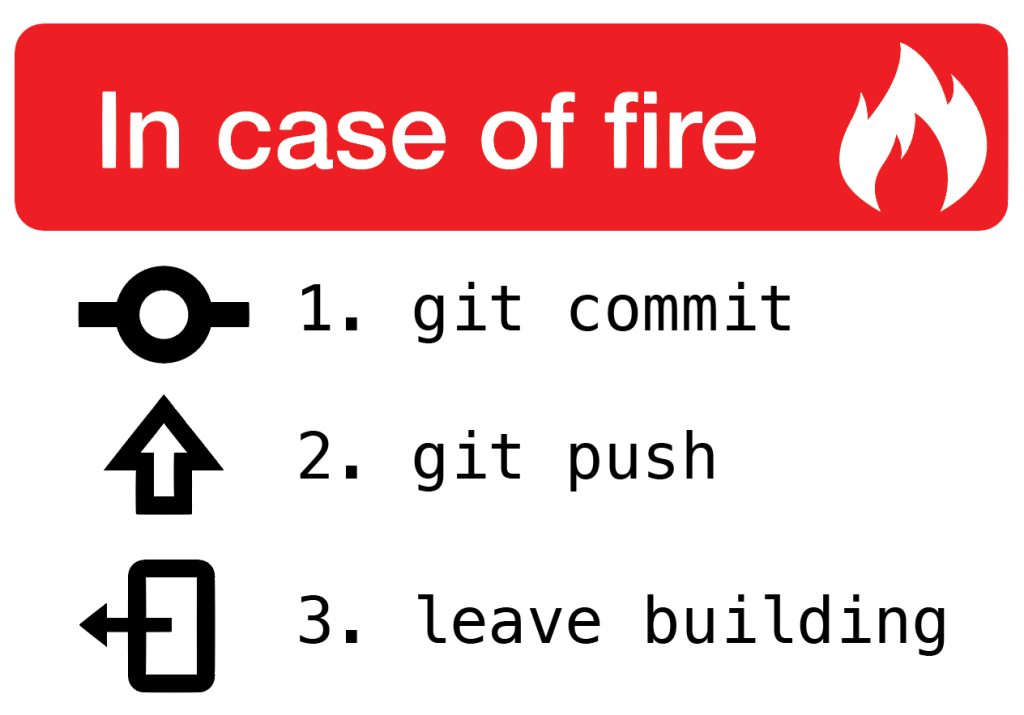
\includegraphics[scale=0.5]{images/incaseoffire.png}
    \end{center}
  \end{columns}
\end{frame}

% \begin{frame}{Trabajar con Remotos - Seguimiento}
%   \begin{itemize}
%     \item \alert{Crear una rama de seguimiento}
%       \mint{console}| $ git checkout --track <remoto>/<rama>|
%       {\scriptsize La rama se llamará \texttt{<rama>} y nos moveremos a ella}
%       \mint{console}| $ git checkout -b <rama> <remoto>/<rama>|
%     \item \alert{Asignar seguimiento a una rama creada}
%       \mint{console}| $ git branch -u <remoto>/<rama>|
%     \item \alert{Ver las ramas a la que hace seguimiento}
%       \mint{console}| $ git branch -vv|
%   \end{itemize}
%   Cuando hacemos \texttt{clone}, automáticamente \texttt{master} hace seguimiento de \texttt{origin/master}
% \end{frame}
